\documentclass[12pt, a4paper, twoside]{article}

%% Preamble
\usepackage{umatfgspanish}
\usepackage{tabto}
\newcommand\ttab{\tab \hspace{-5cm}}
\graphicspath{{./images/}}

\begin{document}
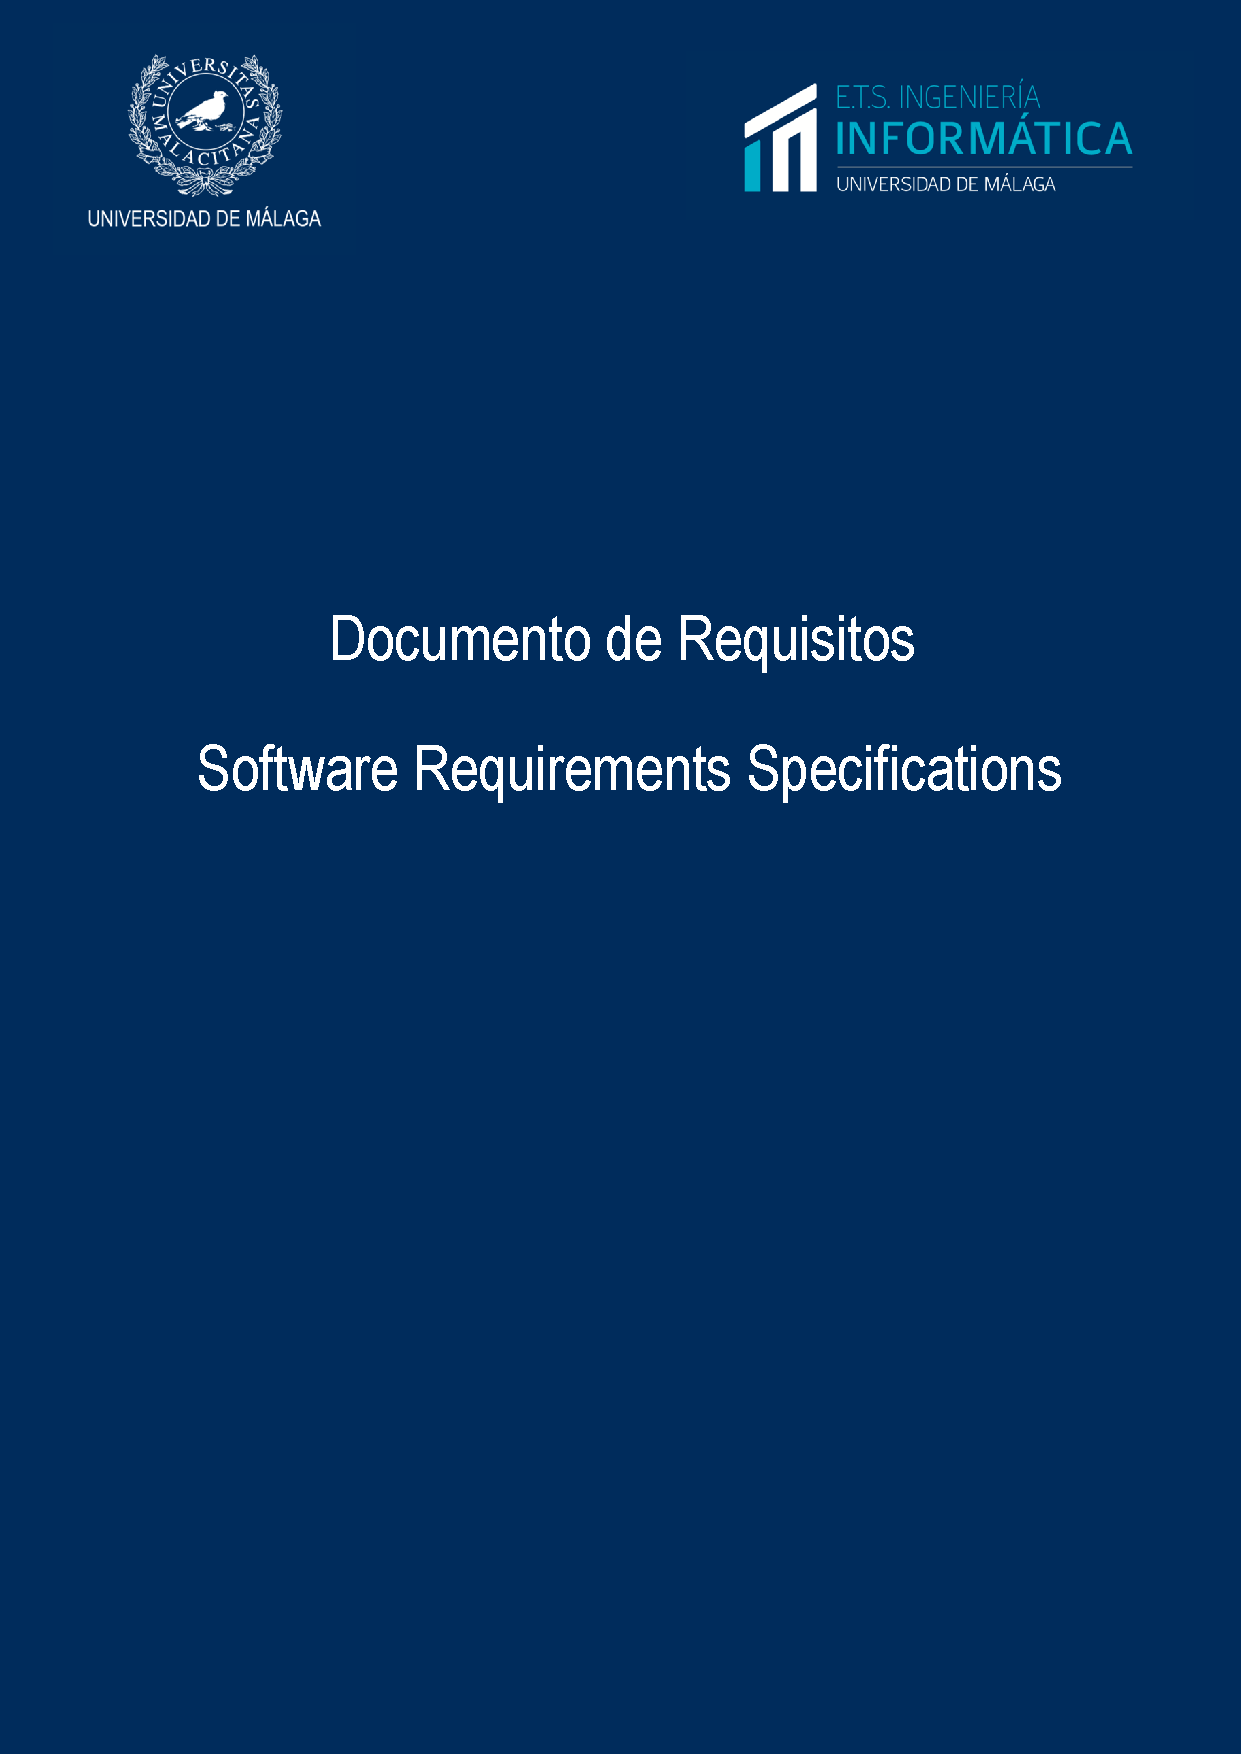
\includepdf[noautoscale=true, width=\paperwidth]{title.pdf}
\newpage
\tableofcontents

%% Sections
\section{Introducción}
\subsection{Propósito}
Desarrollar una plataforma virtual común que permita:
\begin{itemize}
  \item Gestionar y organizar la información de cualquier edificio 
        dentro de una ciudad.
  \item Interconectar cualquier elemento integrable a la red de Internet 
        (dispositivos IoT) que se encuentren en un edificio (Smart Building)
        usando interfaces de comunicación que ya son estándar.
\end{itemize}

\subsection{Ámbito}
Debido a las características del software que hacen uso de las tecnologías 
``Internet de las Cosas'' (IoT) para la gestión de dispositivos conectados a
la red de un Edificio Inteligente (Smart Building), se ha decidido darle el nombre de
``IBuilding''.

% META
IBuilding pretende ser un gestor de los edificios de una ciudad con el que
poder consultar información sobre ellos y manipular sus dispositivos.
 
 % OBJETIVO
Para ello, IBuilding deberá almacenar datos de los edificios y 
deberá disponer de herramientas para acceder y manipular los dispositivos que se instalen
en los mismos.

% Beneficio
De esta manera, se puede enriquecer el valor de una ciudad, permitiendo digitalizar más
datos sobre ella y poder generar una información más fiel y útil para que otras personas
y servicios digitales puedan hacer uso de ella.

IBuilding dispondrá de un servidor central (llamado DataBuilding) que, usando la tecnología
de Fiware, almacenará los datos propios de cada edificio (como la ubicación o el 
tipo de servicio que ofrecen) y los dispositivos disponibles en el mismo. 
Se podrán consultar los datos a través de una API que usará modelos estándares 
de datos.

Los diferentes dispositivos necesitarán controladores que permitan conectarse
a internet para poder manipularlos mediante algún API.

Como ejemplo se desarrollarán algunos Controllers, para hacer uso y alimentar a la API.
Estos dotarán a los dispostivos (Ya sean físicos o virtuales) de acceso a internet, usando interfaces 
estándares, como UltraLight 2.0, OneM2M o directamente NGSI-LD. Ejemplos de Controllers podrían
ser SensorController o ANNPlateController.

El desarrollo de una interfaz de usuario puede ser útil para la gestión de la plataforma
a nivel usuario. Es por eso que también habrá un frontal para hacer uso de IBuilding
que se conectará al DataBuilding y podrá visualizar/modificar los datos oportunos.
Para referirnos a este frontal usaremos el nombre de FrontalBuilding.

% Describe the scope of the software under consideration by:
% a) identifying the software product(s) to be produced by name (e.g., Host DBMS, Report Generator, etc.);
% b) explaining what the software product(s) will do;
% c) describing the application of the software being specified, including relevant benefits, objectives
% and goals; and
% d) being consistent with similar statements in higher-level specifications (e.g., a system requirements
% specification), if they exist.

\section{Visión general del producto}
\subsubsection{Perspectiva del Producto}
Desde el punto de visto externo, IBuilding puede ser visto como un servicio de integración que
\begin{itemize}
  \item ofrezca datos sobre los edificio a aplicaciones terceras.
  \item permita controlar dispositivos mediante una API estándar y conocida.
  \item permita conectar dispositivos IoT de la Smart Building a la red.
\end{itemize}

Para la implementación de esta interfaz Fiware es un candidato óptimo, ya que ofrece NGSI-LD,
una interfaz de comunicación reconocida por diferentes organismo importantes de referencia en toda la Unión Europea.

Además, Fiware deja abierta la posiblidad de implementar otras interfaces que se usan en desarrollo de dispositivos
IoT como UltraLight 2.0 o OneM2M, que también se considera un estándar reconocido por organismos
como la ETSI.

\begin{figure}[h]
  \centering
  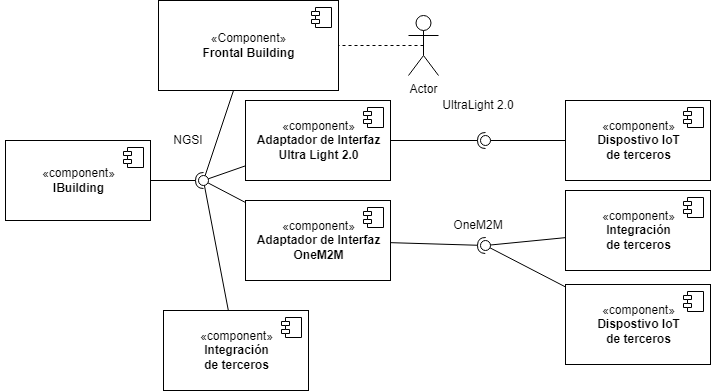
\includegraphics[width=0.8\textwidth]{IBuildingGenericComponents.1.1.png}
  \caption{Niveles de integración posibles siguiendo una aproximación con Gemelo Digital}
\end{figure}
% Define the system's relationship to other related products.
% If the product is an element of a larger system, relate the requirements of that larger system to the
% functionality of the product covered by the SRS.
% If the product is an element of a larger system, identify the interfaces between the product covered by
% the SRS and the larger system of which the product is an element.
% Consider a block diagram showing the major elements of the larger system, interconnections and
% external interfaces.

\subsubsection{Interfaces de Usuario}
% Specify the logical characteristics of each interface between the software product and its users.
% NOTE A style guide for the user interface can provide consistent rules for organization, coding and
% interaction of the user with the system.

\subsubsection{Interfaces Hardware}
% Specify the logical characteristics of each interface between the software product and the hardware
% elements of the system. This includes configuration characteristics (number of ports, instruction sets,
% etc.). It also covers such matters as what devices are to be supported, how they are to be supported, and
% protocols. For example, terminal support may specify full-screen support as opposed to line-by-line
% support.

\subsubsection{Interfaces Software}
Para poder afirmar que un sistema está impulsado por Fiware, es necesario incluir un Context Broker del catálogo de Fiware.
Se ha elegido Orion-LD Context Broker, por implementar la interfaz NGSI-LD y por sus características de tamaño.

Además, por cuestiones de Seguridad, también se incluirán IdM Keyrock y Wilma, que son softwares completamente integrables y
compatibles con NGSI-LD. 

También se incluirá FogFlow como solución para orquestar flujos de trabajos que involucren a los dispositivos IoT. Esta solución 
se beneficia de la computación en el borde para optimizar llamadas innecesarias a servidores y ahorrar tiempo y dinero por ahorro
de cómputos en servidores en la nube. Este servicio también tiene compatibilidad con NGSI-LD.

Como último, se incluirán los IoT Agents: Softwares de Fiware que se encargan de adaptar la interfaz NGSI-LD a otros protocolos
e interfaces para poder ampliar las interfaces de comunicación que se ofrecen. Los IoT Agents que se van a incluir en este proyecto
son IoT Agent - Ultralight 2.0 y OpenMTC.
\begin{center}
  \begin{tabular}{ |c|c|c|c|c| } 
   \hline
   Nombre                     & Abreviatura & Última Versión & Interfaz Relevante & Fuente \\ \hline
   Orion-LD Context Broker    & OCB         & 1.1.2          & NGSI-LD            & https://github.com/FIWARE/context.Orion-LD \\ \hline 
   Identity Manager - Keyrock & IdM Keyrock & 8.3.1          & IdM GE API         & https://github.com/ging/fiware-idm \\ \hline
   PEP Proxy - Wilma          & Wilma       & 8.3            & NGSI-LD            & https://github.com/ging/fiware-pep-proxy \\ \hline
   FogFlow                    & FogFlow     & 3.2.8          & NGSI-LD            & https://github.com/smartfog/fogflow \\ \hline
   IoT Agent - Ultralight 2.0 & IotAgentUL  & 1.23.0         & Ultralight 2.0     & https://github.com/telefonicaid/iotagent-ul \\ \hline
   OpenMTC                    & OpenMTC     & 1.3.0          & OneM2M             & https://github.com/OpenMTC/OpenMTC \\ \hline
  \end{tabular}
\end{center}

\subsubsubsection{NGSI-LD}
// Explicación de NGSI-LD
\subsubsubsection{IdM GE API}
https://keyrock.docs.apiary.io/

https://keyrock-fiware.github.io
\subsubsubsection{Ultralight 2.0}
\subsubsubsection{OneM2M}
% Specify the use of other required software products (e.g., a data management system, an operating
% system or a mathematical package), and interfaces with other application systems (e.g., the linkage
% between an accounts receivable system and a general ledger system).
% For each required software product, specify: name;  mnemonic; specification number; version number; and source.
% NOTE It is acceptable to specify required platforms or operating systems, but rarely feasible to require a
% specific version. Typically, a version number most recent version or any currently maintain version can be
% specified for software.
% For each interface, specify:
% a) discussion of the purpose of the interfacing software as related to this software product;
% b) definition of the interface in terms of message content and format. It is not necessary to detail any
% well-documented interface, but a reference to the document defining the interface is required.

\subsubsection{Interfaces de Comunicación}
Specify the various interfaces to communications such as local network protocols.

\subsubsection{Restricciones de Memoria}
Specify any applicable characteristics and limits on primary and secondary memory.

\subsubsection{Operaciones}
Specify the normal and special operations required by the user such as:
a) the various modes of operations in the user organization (e.g., user-initiated operations);
b) periods of interactive operations and periods of unattended operations;
c) data processing support functions; and
d) backup and recovery operations.
NOTE This is sometimes specified as part of the User Interfaces section.

\subsubsection{Site adaptation requirements}
The site adaptation requirements include:
a) definition of the requirements for any data or initialization sequences that are specific to a given
site, mission or operational mode (e.g., grid values, safety limits, etc.);
b) specification of the site or mission-related features that should be modified to adapt the software
to a particular installation.

\subsubsection{Interfaces with services}
Specify interactions with services, e.g., Software as a Service (SaaS) or cloud services.


\section{Funciones del producto}
Provide a summary of the major functions that the software will perform. For example, an SRS for an
accounting program may use this part to address customer account maintenance, customer statement
and invoice preparation without mentioning the vast amount of detail that each of those functions
requires.
Sometimes the function summary that is necessary for this part can be taken directly from the section
of the higher-level specification (if one exists) that allocates particular functions to the software
product.
Use cases, user stories and scenarios are also used to describe product functions.
Note that for the sake of clarity:
a) the product functions should be organized in a way that makes the list of functions understandable
to the acquirer or to anyone else reading the document for the first time.
b) textual or graphical methods can be used to show the different functions and their relationships.
Such a diagram is not intended to show a design of a product, but simply shows the logical
relationships among variables.

 \subsubsection{Características de los Usuarios}
 Describe those general characteristics of the intended groups of users of the product including
 characteristics that may influence usability, such as educational level, experience, disabilities and
 technical expertise. This description should not state specific requirements, but rather should state the
 reasons why certain specific requirements are later specified in specific requirements in 9.6.9.
 NOTE 1 Where appropriate, the user characteristics of the SyRS and SRS are consistent.
 NOTE 2 For additional information on context of use and user needs, see ISO/IEC 25063 and ISO/IEC 25064.

 \subsubsection{Limitaciones}
 Provide a general description of any other items that will limit the supplier's options, including:
 a) regulatory requirements and policies;
 b) hardware limitations (e.g., signal timing requirements);
 c) interfaces to other applications;
 d) parallel operation;
 e) audit functions;
 f) control functions;
 g) higher-order language requirements;
 h) signal handshake protocols (e.g., XON-XOFF, ACK-NACK);
 i) quality requirements (e.g., reliability);
 j) criticality of the application;
 k) safety and security considerations;
 l) physical/mental considerations; and
 m) limitations that are sourced from other systems, including real-time requirements from the
 controlled system through interfaces.

\subsection{Definiciones}
\begin{itemize}
    \item \textbf{Sensores}\ttab Los sensores son dispositivos IoT cuya labor principal es recolectar datos.
    \item \textbf{Actuadores}\ttab Los actuadores son dispositivos IoT cuya función principal hacer una tarea.
\end{itemize}

\section{Referencias}

\section{Requisitos}
\subsection{Funciones}
Define the fundamental actions that have to take place in the software in accepting and processing the
inputs and in processing and generating the outputs, including:
a) validity checks on the inputs;
b) exact sequence of operations;
c) responses to abnormal situations, including:
1) overflow;
2) communication facilities;
3) hardware faults and failures; and
4) error handling and recovery;
d) effect of parameters;
e) relationship of outputs to inputs, including:
1) input/output sequences; and
2) formulas for input to output conversion.
It may be appropriate to partition the functional requirements into sub-functions or sub-processes.
This does not imply that the software design will also be partitioned that way.

\subsection{Requisitos de Rendimiento}
Specify both the static and the dynamic numerical requirements placed on the software or on human
interaction with the software as a whole.
Static numerical requirements may include the following:
a) the number of terminals to be supported;
b) the number of simultaneous users to be supported; and
c) the amount and type of information to be handled.
Static numerical requirements are sometimes identified under a separate section entitled Capacity.
Dynamic numerical requirements may include, for example, the numbers of transactions and tasks and
the amount of data to be processed within certain time periods for both normal and peak workload
conditions.
The performance requirements should be stated in measurable terms.
For example,
95 \% of the transactions shall be processed in less than 1 s.
rather than,
An operator shall not have to wait for the transaction to complete.
NOTE Numerical limits applied to one specific function are normally specified as part of the processing
subparagraph description of that function.

\subsection{Requisitos de Usabilidad}
Define usability and quality in use requirements and objectives for the software system that can include
measurable effectiveness, efficiency, satisfaction criteria and avoidance of harm that could arise from
use in specific contexts of use.
NOTE Additional guidance on usability requirements can be found in ISO/IEC TR 25060.

\subsection{Requisitos de Interfaces}

 \subsubsection{Interfaces externas}
 Define all inputs into and outputs from the software system. The description should complement the
 interface descriptions in 9.6.4.1 through 9.6.4.5, and should not repeat information there.
 Each interface defined should include the following content:
 a) name of item;
 b) description of purpose;
 c) source of input or destination of output;
 d) valid range, accuracy and/or tolerance;
 e) units of measure;
 f) timing;
 g) relationships to other inputs/outputs;
 h) data formats;
 i) command formats; and
 j) data items or information included in the input and output.

 \subsection{Logical database requirements}
 Specify the logical requirements for any information that is to be placed into a database, including:
 a) types of information used by various functions;
 b) frequency of use;
 c) accessing capabilities;
 d) data entities and their relationships;
 e) integrity constraints;
 f) security; and
 g) data retention requirements.

 \subsection{Restricciones de Diseño}
 Specify constraints on the system design imposed by external standards, regulatory requirements or
 project limitations.

 \subsection{Software system attributes}
 Specify the required attributes of the software product. The following is a partial list of examples:
 a) Reliability - specify the factors required to establish the required reliability of the software system
 at the time of delivery.
 b) Availability - specify the factors required to guarantee a defined availability level for the entire
 system such as checkpoint, recovery and restart.
 c) Security - specify the requirements to protect the software from accidental or malicious access,
 use modification, destruction or disclosure. Specific requirements in this area could include the
 need to:
 1) utilize certain cryptographic techniques;
 2) keep specific log or history data sets;
 3) assign certain functions to different modules;
 4) restrict communications between some areas of the programme;
 5) check data integrity for critical variables; and
 6) assure data privacy.
 d) Maintainability - specify attributes of software that relate to the ease of maintenance of the
 software itself. These may include requirements for certain modularity, interfaces or complexity
 limitation. Requirements should not be placed here just because they are thought to be good design
 practices.
 e) Portability - specify attributes of software that relate to the ease of porting the software to other
 host machines and/or operating systems, including:
 1) percentage of elements with host-dependent code;
 2) percentage of code that is host dependent;
 3) use of a proven portable language;
 4) use of a particular compiler or language subset; and
 5) use of a particular operating system.

 \subsection{Información de Soporte}
 Additional supporting information to be considered includes:
 a) sample input/output formats, descriptions of cost analysis studies or results of user surveys;
 b) supporting or background information that can help the readers of the SRS;
 c) a description of the problems to be solved by the software; and
 d) special packaging instructions for the code and the media to meet security, export, initial loading
 or other requirements.
 The SRS should explicitly state whether or not these information items are to be considered part of the
 requirements.

 \section{Apportioning of requirements???}
 Apportion the software requirements to software elements. For requirements that will require
 implementation over multiple software elements, or when allocation to a software element is initially
 undefined, this should be so stated. A cross-reference table by function and software element should be
 used to summarize the apportionments.
 Identify requirements that may be delayed until future versions of the system (e.g., blocks and/or
 increments).

 \section{Specified requirements???}
 Specify the software system requirements to a level of detail sufficient for software design, development
 and verification of the software increment or release in process.
 The requirements should:
 a) be stated in conformance with all the characteristics described in 5.2 of this document;
 b) be cross-referenced to earlier versions or related documents;
 c) be uniquely identifiable;
 d) describe every input (stimulus) into the software system, every output (response) from the
 software system, and all functions performed by the software system in response to an input or in
 support of an output.

 \section{Standards compliance???}
 Specify the requirements derived from existing standards or regulations, including:
 a) report format;
 b) data naming;
 c) accounting procedures; and
 d) audit tracing.
 For example, this could specify the requirement for software to trace processing activity. Such traces
 are needed for some applications to meet minimum regulatory or financial standards. An audit trace
 requirement may, for example, state that all changes to a payroll database shall be recorded in a trace
 file with before and after values.

 \section{Verificación}
 Provide the verification approaches and methods planned to qualify the software. The information
 items for verification are recommended to be given in a parallel manner with the information items in
 9.6.10 to 9.6.18.

\section{Apéndice}
\subsection{Suposiciones y dependencias}
List each of the factors that affect the requirements stated in the SRS. These factors are not design
constraints on the software but any changes to these factors can affect the requirements in the SRS.
For example, an assumption may be that a specific operating system will be available on the hardware
designated for the software product. If, in fact, the operating system is not available, the SRS would
have to change accordingly.
\subsection{Acrónimos y Abreviaturas}
\begin{itemize}
    \item \textbf{IoT}\ttab Internet de las Cosas.
    \item \textbf{API}\ttab Application Program Interface.
  \end{itemize}


\end{document}